% TODO:
% - clarify relation with Marsi et al 2014
% - explicitly point out new contributions
% - stress there are no existing systems or benchmarks to compare to (evaluation)
% - The main objective of the paper is not very clear: is it to propose the dataset
%    or to describe the methodology to obtain it automatically ? or both?
% - stress that this is ongoing work, so no evaluation yet
 



\documentclass[11pt]{article}
\usepackage{acl2015}
\usepackage{times}
\usepackage{url}
\usepackage{latexsym}
\usepackage{graphicx}
\usepackage{amsmath}  
\usepackage{array}

\usepackage{booktabs}
\usepackage{placeins}

%\setlength\titlebox{5cm}

% You can expand the titlebox if you need extra space
% to show all the authors. Please do not make the titlebox
% smaller than 5cm (the original size); we will check this
% in the camera-ready version and ask you to change it back.

\DeclareMathSizes{9}{8}{7}{6}
\renewcommand{\floatpagefraction}{1.0}%

\title{Extraction and generalisation of variables from scientific publications}

\author{Erwin Marsi, Pinar \"Ozt\"urk\\
  Department of Computer and Information Science\\
  Norwegian University of Science and Technology (NTNU)\\
  {\tt \{emarsi,pinar\}@idi.ntnu.no}}
  
\date{}

\begin{document}
\maketitle

\begin{abstract}

Scientific theories and models in Earth science typically involve changing \emph{variables} and their complex interactions, including correlations, causal relations and chains of positive/negative feedback loops. 
Variables tend to be complex rather than atomic entities and expressed as noun phrases containing multiple modifiers, e.g. \emph{oxygen depletion in the upper 500 m of the ocean or timing} and \emph{magnitude of surface temperature evolution in the Southern Hemisphere in deglacial proxy records}.
Text mining from Earth science literature is therefore significantly different from biomedical text mining and requires different approaches and methods.
Our approach aims at automatically locating and extracting variables and their direction of variation: \emph{increasing}, \emph{decreasing} or just \emph{changing}.
Variables are initially extracted by matching tree patterns onto the syntax trees of the source texts.
Next, variables are generalised in order to enhance their similarity, facilitating hierarchical search and inference.
This generalisation is accomplished by progressive pruning of syntax trees using a set of tree transformation operations.
Text mining results are presented as a browsable variable hierarchy which allows users to inspect all mentions of a particular variable type in the text as well as any generalisations or specialisations.
The approach is demonstrated on a corpus of 10k abstracts of Nature publications in the field of Marine science.
We discuss experiences with this early prototype and outline a number of possible improvements and directions for future research.
\end{abstract}


%====================================================================================
\section{Introduction}
%====================================================================================

Text mining of scientific literature originates from efforts to cope with the ever growing flood of publications in biomedicine \cite{Swanson1986Fish,Swa88,Swanson1997Interactive,Hearst:1999aa,Ananiadou2006,Zweigenbaum2007Frontiers,Cohen2005Survey,Krallinger2008Linking,RodriguezEsteban2009Biomedical,Zweigenbaum2009Advanced,Ananiadou2010Event,Simpson2012Biomedical,ananiadou2014event}.
Consequently the resulting approaches, methods, tools and applications -- as well as data, corpora and evaluation tasks -- are rooted in the paradigm of biomedical research and its conceptual framework.
Typical source text consists of abstracts from PubMed or full-text articles from PubMed Central.
Standard tasks include recognition, normalisation and mapping of biological entities (e.g., genes, proteins, drugs, symptoms and diseases), extraction of biological relations (e.g., protein-protein interaction, disease-gene associations or drug-drug interaction) or bio-event extraction (e.g., regulation or inhibition events and their participants). 
There are extensive ontologies like the Gene Ontology \cite{ConsortiumTheGeneOntology2001Creating}, annotated corpora like the GENIA \cite{Kim2003GENIA} and BioInfer \cite{Pyysalo:2007} corpora and  dedicated shared tasks including BioCreative \cite{Hirschman2005Overview} and BioNLP \cite{Pyysalo2012Overview}.
In short, there is a whole infrastructure supporting biomedical text mining \cite{Cohen2008Getting}.

Text mining is now spreading out to other scientific disciplines, notably in the humanities and social sciences \cite{oconnor2011}, holding the promise for knowledge discovery from large text collections.
Our own research targets text mining in the field of Earth science, more specifically in Oceanography or Marine science, with a focus on climate change.
As text mining efforts in this area are extremely rare \cite{ekstrom2008exploratory,vossen-EtAl:2010:ONTOLEX,Zhang2013GeoDeepDive,marsi2014towards,aamot2014literature}, it is not surprising that a corresponding infrastructure is mostly lacking.
In addition, however, we found that due to significant differences between the conceptual frameworks of biomedicine and marine science, simply ``porting" the biomedical text mining infrastructure to another domain will not suffice.

One major difference is that the biomedical entities of interest are relatively well defined -- genes, proteins, organisms, species, drugs, diseases, etc. -- and typically expressed as proper nouns.
In contrast, defining the entities of interest in marine science turns out to be much harder.
Not only does it seem to be more open-ended in nature, the entities themselves tend to be complex and expressed as noun phrases containing multiple modifiers, giving rise to examples like \emph{oxygen depletion in the upper 500 m of the ocean} or \emph{timing and magnitude of surface temperature evolution in the Southern Hemisphere in deglacial proxy records}.

Given the difficulties with entities, 
%in the marine science domain, 
we propose to concentrate first on text mining of events, leaving entities underspecified for the time being. 
Theories and models in marine science are characterised by changing variables and their complex interactions, including correlations, causal relations and chains of positive/negative feedback loops.
Many marine scientists are interested in finding evidence -- or counter-evidence -- in the literature for events of change and their relations.    
Here we present ongoing work to automatically locate and extract \emph{variables} and their direction of variation: \emph{increasing}, \emph{decreasing} or just \emph{changing}. 
Examples are given in Table~\ref{tab:variables}.

Since many of these changing variables are long and complex expressions, their frequency of occurrence tends to be low, making the discovery of relations among different variables harder.
As a partial solution to this problem, we propose progressive pruning of syntax trees using a set of tree transformation operations.
For example, generalising \emph{oxygen depletion in the upper 500 m of the ocean} to \emph{oxygen depletion in the ocean} and subsequently to the much more frequent \emph{oxygen depletion}.
Text mining results are then presented as a browsable variable hierarchy which allows users to inspect all mentions of a particular variable type in the text as well as any generalisations or specialisations. 
   

\begin{table*}[tb]
\caption{Examples of tree patterns and matching variables}
\begin{center}
\begin{small} 
\begin{tabular*}{\textwidth}{l p{5.3cm} p{8.2cm}}
\toprule
\textbf{Direction}: & \text{\textbf{Tree pattern:}} & \textbf{Matched variable in sentence:} \\
\midrule

Change   & \vspace{-11pt} 
\begin{verbatim}NP <- (/NN/=d1 < variability 
$ /NN/) !$. PP\end{verbatim} &
Thus \textbf{the annual, Milankovitch and continuum temperature variability} together represent the response to deterministic insolation forcing. \\

\midrule
\vspace{-11pt} 
Increase & 
 \vspace{-11pt} 
\begin{verbatim}NP > (PP <<# (in|of) $, 
(NP <<# increase)) \end{verbatim} & 
The record reveals a linear increase in \textbf{annual temperature between 1958 and 2010} by 2.4 +/-1.2 degreesC \ldots \\
\midrule

Decrease  &  \vspace{-11pt} 
\begin{verbatim}NP > (VP <<# reduce )\end{verbatim}  &
 Some researchers have observed that abundant natural gas substituting for coal could reduce \textbf{carbon dioxide (CO2) emissions}.  \\

\bottomrule
\end{tabular*}
\end{small}
\end{center}
\label{tab:variables}
\vspace{-3mm}
\end{table*}%


%====================================================================================
\section{Variable extraction}
%====================================================================================

%Our text material consists of abstracts from journals published by Nature Publishing Group, constructed in the following way.
%First a panel of three domain experts supplied us with a number of survey articles in the area of interest, i.e., the biological pump, the microbial food web and their relation to climate change.
%Terms were automatically extracted using the TerMine webservice \cite{Frantzi2000} and the top-n terms were subsequently judged by the panel as relevant or not.
%Each of the resulting 305 terms was then used to query the Nature's OpenSearch API\footnote{\url{http://www.nature.com/developers/documentation/api-references/opensearch-api}} for publications in a limited range of relevant journals, after 1997, retrieving records including title and abstract.
%Retrieval results were ranked according to the number of search terms they matched. 
%We selected the top 10k abstracts for further processing with CoreNLP pipeline \cite{manning-EtAl:2014:P14-5}, including  tokenisation, sentence splitting, POS tagging, lemmatisation and parsing.
%Lemmatised parse trees were created by substituting terminals with their lemmas.
%The resulting corpus contains 9,586 article abstracts, 59,787 sentences and approximately 4M tokens.

Our text material consists of 10k abstracts from journals published by Nature Publishing Group.
Search terms obtained from domain experts were used to query Nature's OpenSearch API\footnote{\url{http://www.nature.com/developers/documentation/api-references/opensearch-api}} for publications in a limited range of relevant journals, after 1997, retrieving records including title and abstract.
The top-10k abstracts matching most search terms were selected for further processing with CoreNLP \cite{manning-EtAl:2014:P14-5}, including  tokenisation, sentence splitting, POS tagging, lemmatisation and parsing.
Lemmatised parse trees were obtained by substituting terminals with their lemmas.
The resulting new corpus contains 9,586 article abstracts, 59,787 sentences and approximately 4M tokens.

Methods for information extraction broadly rely on either knowledge-based pattern matching or supervised machine learning \cite{Sarawagi:2008:IE:1498844.1498845}.
Although ML approaches are currently dominant in IE research, rule-based systems have several advantages, including: (a) the rules are interpretable and thus suitable for rapid development and domain transfer; and (b) humans and machines can contribute to the same model \cite{Valenzuela-Escarcega:2015aa}.
%Both approaches have their advantages and disadvantages, but both require a similar investment of time and effort in either writing patterns or manual annotation of training examples. 
%Our initial experiments suggested somewhat better performance was obtained with pattern matching.     
%In addition,
In our case, patterns offered more flexibility in exploring the domain, whereas the manual annotation required for ML demands more commitment to a precise definition of entities, relations and events, which we found hard to achieve at this stage.
%Hence the choice for pattern matching on syntax trees is pragmatic rather than dogmatic.
Tree pattern matching is applied to lemmatised syntax trees using the Tregex engine \cite{Levy2006}, which supports a compact language for writing regular expressions over trees; 
see Table~\ref{tab:variables} for examples of patterns and matching phrases.
% refs to earlier work?
% motivation for syntax?
For instance, the pattern for a decreasing variable is defined as a noun phrase (NP) that is immediately dominated (\verb|>|) by a verb phrase (VP), which in turn is headed by (\verb|<<#|) the lemma \emph{reduce}.
Similarly, the pattern for increase describes an NP dominated by a prepositional phrase (PP) that is headed by the preposition \emph{in} or \emph{of}; in addition, this PP must be preceded by an NP sister node (\verb|$,|) headed by the lemma \emph{increase}.

Patterns were generated by instantiating a small set of hand-written pattern templates, drawing from manually created lists of verbs and nouns expressing change, increase or decrease. 
The patterns cover expression as a main verb (\emph{X increases, something increases X)}, attributive use of verbs (\emph{increasing temperature, temperature is increasing}), head of NP (\emph{a temperature increase}) or NP with PP modifier (\emph{increase in temperature}).
The total number of patterns is 320: 90 for change, 122 for increase, 108 for decrease (see supplements for a full list).
The total number of matched variables in the corpus is 21,817: 9,352 for change, 7,400 for increase and 5,065 for decrease.

Some variables do not exactly correspond to a node, i.e., not every variable is a valid syntactic phrase.
For instance, the pattern for Change in Table~\ref{tab:variables} matches the NP \emph{the annual, Milankovitch and continuum temperature variability}, whereas the actual variable is \emph{the annual, Milankovitch and continuum temperature}.
This is corrected in a post-processing step that deletes the \emph{variability} node from the extracted subtree and substring.
For this purpose, the pattern contains an assignment of the name d1 to the node directly dominating the lemma \emph{variability} (\verb|/NN/=d1 < variability|)), allowing a corresponding tree operation to delete this node, which is implemented using the Tsurgeon counterpart of Tregex.
 
%====================================================================================
\section{Variable generalisation}
%====================================================================================

Since many of the extracted variables are long and complex expressions, their frequency is low.
The most frequent variables are generic terms (\emph{climate} 1207,  \emph{temperature} 156, \emph{global climate} 73), but over 66\% is unique.
This evidently impedes the discovery of relations among variables.
As a partial solution to this problem, variables are generalised by progressive pruning of syntax trees using a set of tree transformation operations.

Figure~\ref{fig:gen} shows an example of generalisation by iterative tree pruning.
The first transformation \textsc{Strip Init DT}  strips the initial determiner from the NP.
Next,  \textsc{Coord 3.1}  deletes everything but the first conjunct from a coordinated structure of three NPs, resulting in \emph{annual temperature} , which is finally reduced to just \emph{temperature} by stripping the premodifier (\textsc{Strip Premod 1} ).
An analogous procedure is applied to the other two conjuncts of the coordinated structure.

Tree transformations are implemented using Tsurgeon \cite{Levy2006}: Tregex patterns match the syntactic structures of interest, whereas an associated Tsurgeon operation deletes selected  nodes (see supplements for details).
The transformations are ordered in four groups.
The first group handles coordination of two to four conjuncts (cf. Figure~\ref{fig:gen}) -- at the phrase level or the lexical level -- as well as cases of ellipsis (e.g.  \emph{hailstorm frequency and intensity} into \emph{hailstorm frequency} and \emph{hailstorm intensity}).
The second group strips bracketed material in parenthetical and list structures.
The  third group  deletes non-restrictive relative clauses and other non-restrictive modifiers preceded by a comma.
The final group progressively strips premodifiers (mainly adjectives) from left to right and postmodifiers (PPs, relative clauses) from right to left .
Since different transformation may arrive at the same generalisation  (e.g. \emph{temperature} in Figure~\ref{fig:gen}), duplicates are filtered out.
After filtering, 150,716 variables remained, which is 4.86 times the number of originally extracted variables.
% discuss cyclic application?

As mentioned, the point of generalisation is to find relations among variables.
In Table~\ref{tab:variables}, for example,  both \emph{the annual, Milankovitch and continuum temperature variability } and \emph{annual temperature between 1958 and 2010} are generalised to \emph{annual temperature}.
However, many generalised variables are unique and thus serve no purpose in relating variables.
Retaining only original variables and generalised variables with at least two mentions yields a total of 17,613 variable types. % = len(var_type_index)

\begin{figure}[tb]
\begin{small}
\begin{tabbing}
~~~ \= the annual , Milankovitch and continuum temperature \\
\> ~~~~~~ \= \textsc{Strip Init DT} $\rightarrow$ annual , Milankovitch and \\
\>                                              \>                       continuum temperature \\
\>         \> ~~~~~~ \= \textsc{Coord 3.1} $\rightarrow$  annual temperature \\
\>         \> \> ~~~~~~ \=   \textsc{Strip Premod 1} $\rightarrow$  temperature \\
\>         \> \>  \textsc{Coordi 3.2} $\rightarrow$  Milankovitch temperature \\
\>            \> \> \>         \textsc{Strip Premod 1} $\rightarrow$  temperature \\
\>            \> \> \textsc{Coord 3.3} $\rightarrow$ continuum temperature \\
 \>            \> \> \>        \textsc{Strip Premod 1} $\rightarrow$  temperature \\
\end{tabbing}
\end{small}
%\vspace{-8mm}
\caption{Example of generalisation by iterative tree pruning}
\label{fig:gen}
\end{figure}

%====================================================================================
\section{User interface}
%====================================================================================

\begin{figure*}[!htb]
\setlength\fboxsep{0pt}
\setlength\fboxrule{0.5pt}
%\fbox{
  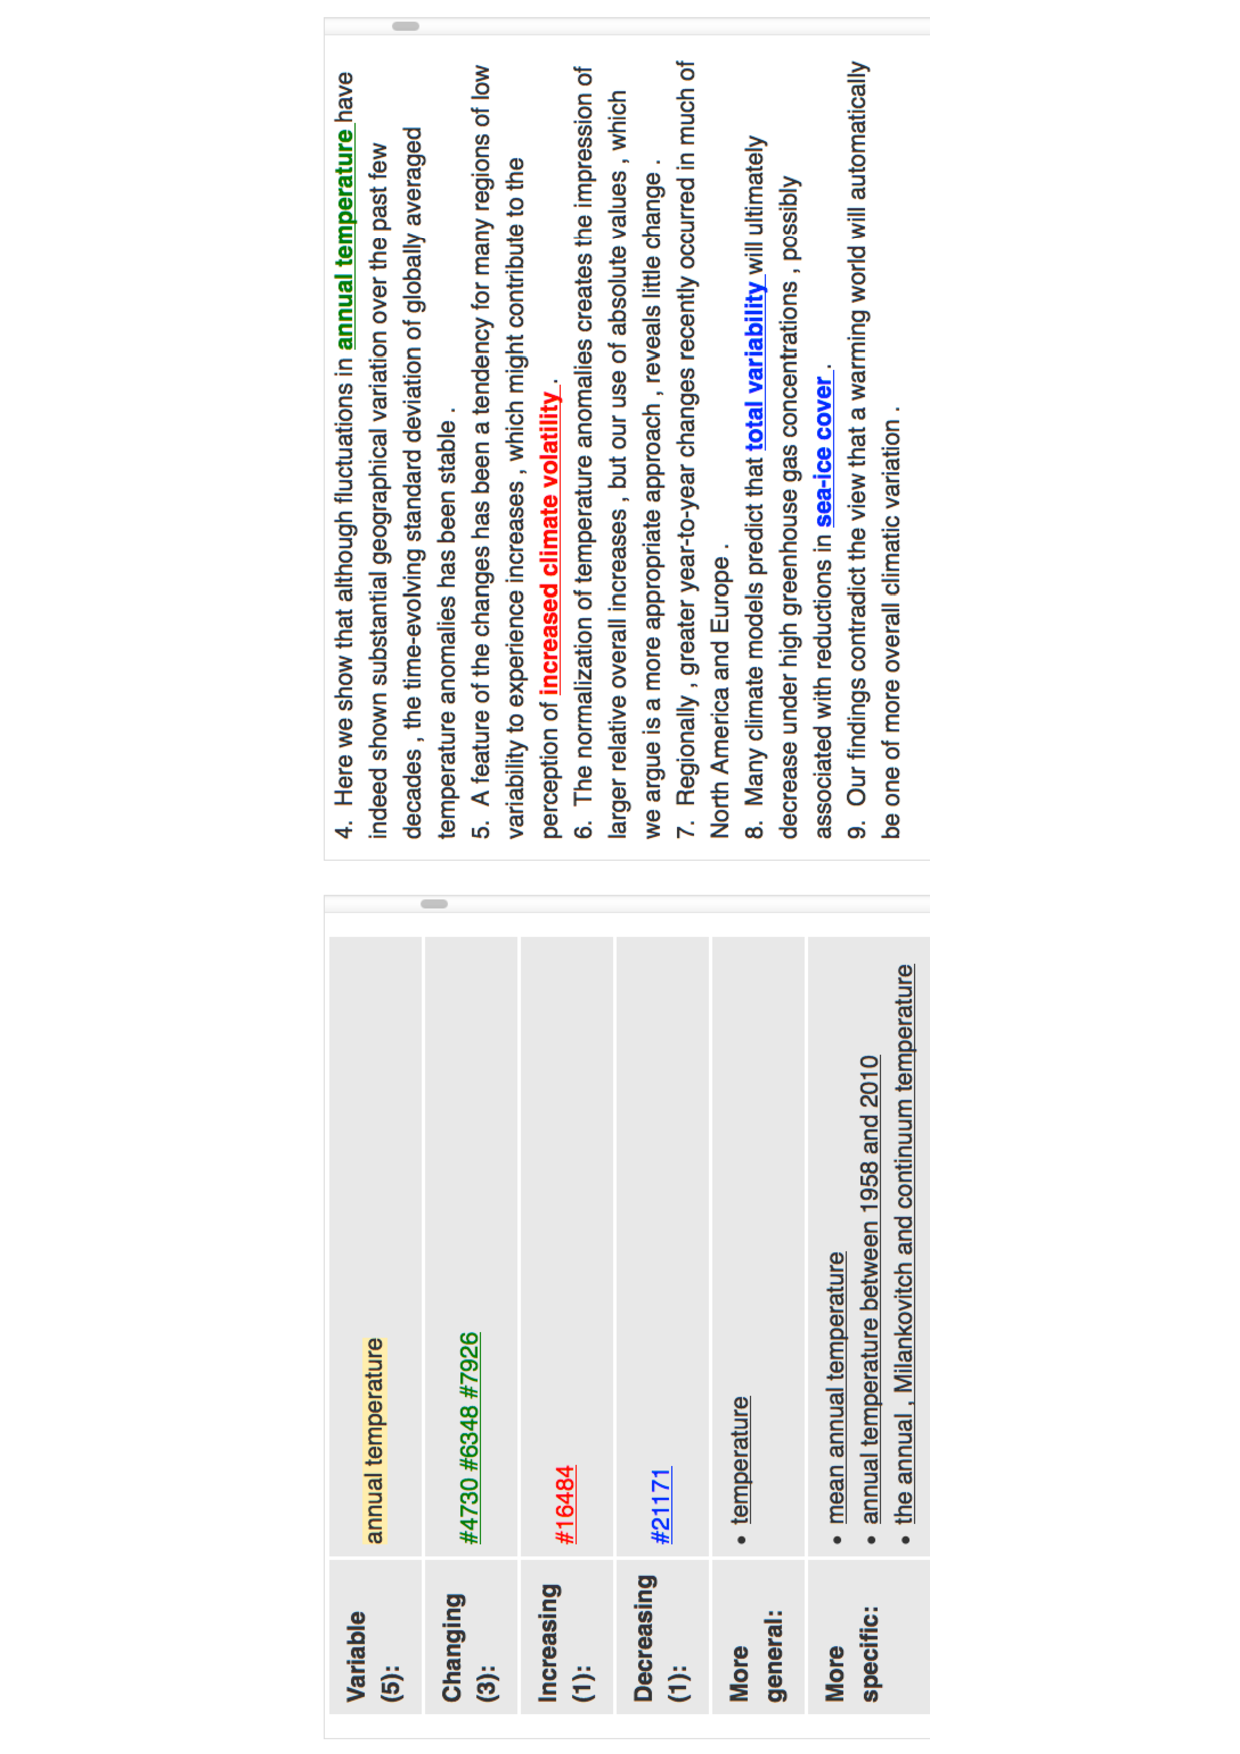
\includegraphics[scale=0.54,angle=-90,clip=true,trim=56mm 1mm 53mm 0]{screenshot.pdf}
  %}
  \caption{Partial screenshot of user interface showing variable type hierarchy (left) and linked variable mentions in text (right)
  where colour encodes change (green), increase (red) or decrease (blue)}
\vspace{4pt}
\label{fig:ui}  
\end{figure*}

The output of the text mining step can be regarded as a directed graph where the nodes are variable \emph{types} and the edges point from a more specific variable to a more general variable (as a result of a particular tree transformation).
Each variable type is also linked to a set of tokens, i.e. variable mentions in the text which are either changing, increasing or decreasing.
Figure~\ref{fig:ui}  shows how this information is presented to the user in a browser (see supplements for full version).
The left panel lists the variable types, ordered from most general to most specific and, secondary, on decreasing token frequency.
Links point to more specific/general variables types, as well as to changing/increasing/decreasing variable mentions in the text.
The right panel shows the source text, where colour encodes changing (green), increasing (red) or decreasing (blue) variable mentions, which are linked to their most specific variable type.
This setup allows users to quickly explore variables, for example, finding abstracts containing a variable of interest and from there to related variables.   
 
%====================================================================================
\section{Discussion}
%====================================================================================

We have argued that the paradigm established in biomedical text mining does not transfer directly to other scientific domains like Earth science.
A new approach was proposed for extracting variables and their direction of variation (increasing, decreasing or just changing), focusing on events rather than entities.
A generic system based on syntactic pattern matching and tree transformations was described for extraction and subsequent generalisation of variable events.
Text mining results are presented in an innovative way as a browsable hierarchy ranging from most general to most specific variables, with links to their textual instances.
In addition, a first text corpus in marine science was produced, including automatically annotated change events.
Our corpus as well as the extracted variables are publicly available\footnote{\url{https://dl.dropboxusercontent.com/u/2370516/emnlp15_corpus.zip}}.
We think our approach to extraction is generalisable to other domains where the entities of interest are common nouns or complex noun phrases rather the proper nouns, e.g. in nanotechnology \& nanoscience \cite{Kostoff20071733}.

To the best of our knowledge, there are currently no other systems for text mining in Earth science which we can compare our results with, nor are there any benchmark data sets for our task.
Most related is \cite{marsi2014towards}, but their definition of variables is more restricted and their pilot corpus is too small for evaluation purposes.
Reporting on our ongoing work now, future work will include an evaluation by asking domain exports to judge the correctness of extracted variables as well as their generalisations in the given context. 

%There is certainly a downside to relying on syntax tree matching. 
Preliminary observations indicate that most problems originate from syntactic parsing errors, in particular well-known ambiguities in coordination and PP-attachment.
As a result, patterns may either fail to match or match unintentionally, yielding incomplete or incoherent variables.     
Since many sentences are long, complex and domain-specific, it comes as no surprise that the parser often fails to correctly resolve well-known ambiguities in coordination and PP-attachment.
However, with pattern matching on strings and/or POS tags instead of syntax trees, determining boundaries of variables would be problematic.
False positives also occur because of different semantics of the same pattern, e.g. \emph{change in western Europe} is unlikely to mean literally that the European continent is changing, neither does \emph{changes in less than a few thousand years} imply that past years are changing.

At the same time, certain false negatives are beyond the power of pattern matching. 
For instance, variation may be entailed rather than explicitly stated:
\emph{ocean acidification} entails increasing acidity of ocean water and \emph{Arctic warming} entails increasing temperature in the Arctic region.
This is closely related to textual entailment \cite{AndroutsopoulosMalakasiotis:2010,DaganGlickmanMagnini:2006}, requiring inference in combination with domain knowledge.
A related matter is negation (\emph{no increase in global temperature}), which can even be expressed in non-trivial ways (\emph{temperature remained constant}) \cite{morante2009learning}.
Variables were also found to be recursive or embedded, expressing ``a change of a change''.  
For example, \emph{reduce subseasonal temperature variance} implies both a change in temperature as well as a decrease of this temperature change.
The current visualisation falls short in these cases, as HTML browsers cannot render a link in a link.

Generalisation by tree pruning appears to work quite well as long as the parse is correct.
However, pruning by itself is insufficient and should be supplemented with other methods.
For instance, linking named entities like species, chemicals or locations to unique concepts in appropriate ontologies/taxonomies would support generalisations such as \emph{iron} is a \emph{metal} or a \emph{diatom} is a \emph{plankton}. 
Generalisation also bears a strong resemblance to other text-to-text generation tasks such as paraphrasing \cite{AndroutsopoulosMalakasiotis:2010}, sentence compression \cite{jing2000sentence} and sentence simplification \cite{shardlow2014survey}.
Given suitable training data,  ML approaches may therefore be applied, e.g. \cite{knight2002,CohnLapata:2009}.

%We are fully aware that in some contexts generalisation is not truth preserving, but to what extent this is a serious problem for knowledge discovery remains to be studied. 
%One important point for future work is therefore evaluation by asking domain exports to judge the correctness of extracted variables as well as their generalisations in the given context. 

The most general variables are probably too generic to be of much help to a user, e.g. \emph{concentration}, \emph{rate}, \emph{level}, etc.
Likewise, \emph{climate} is by far the most frequent changing variable due to the frequently occurring collocation \emph{climate change}.
In addition, variables often contain references to previously mentioned entities -- anaphoric \emph{it} being the ultimate example of this -- suggesting a need for co-reference resolution \cite{Miwa01072012}.

Yet another future direction is to structurally model variables as opposed to a possibly over-simplified generalisation. 
Similar to nominal SRL, one can define relevant arguments including frequency (e.g.
annual), temporal scope (between 1958 and 2010), location, etc.
The most generic variables mentioned earlier in fact provide a good basis for such modelling.

Extraction and generalisation of variables provides a basis for building systems supporting knowledge discovery.
One approach is mining associations between variables frequently co-occurring in the same sentence or abstract \cite{Jenssen:2001aa,Hashimoto2012Excitatory}) 
More precise results can be expected by extracting causal relations between change events \cite{chang2005causal,blanco2008causal,Raja2013PPInterFindera}.
Pairs of change events -- causally or otherwise associated -- obtained from different publications can be chained together, possibly in combination with domain knowledge, in order to generate new hypotheses, as pioneered in the work on literature-based knowledge discovery \cite{Swanson1986Fish,Swa88,Swanson1997Interactive}.
Automatic extraction and generalisation of variables from scientific publications thus paves the way for future research on text mining in Earth science.
 
% Other topics:
% - machine learning approach to IE, annotation required
% - scale up to to full papers
%

\section*{Acknowledgments}

Financial aid from the European Commission (OCEAN-CERTAIN, FP7-ENV-2013-6.1-1; no: 603773) is gratefully acknowledged. 
We thank Murat Van Ardelan for sharing his knowledge of Marine science and the anonymous reviewers for their valuable comments. 



\FloatBarrier 
\pagebreak

\bibliographystyle{acl}
\bibliography{emnlp15_em_po}


\end{document}
